\chapter[Automatic assessment of singing voice pronunciation of jingju music
]{Automatic assessment of singing voice pronunciation of jingju music
}\label{chap:probdef}
% \begin{epigraphs}
% \qitem{A problem well stated is a problem half-solved}{Charles Kettering}
% \qitem{The formulation of the problem is often more essential than its solution, which may be merely a matter of mathematical or experimental skill}{Albert Einstein}
% \end{epigraphs}

Automatic assessment of singing voice of jingju music has not been explored systematically, which means that the challenges, opportunities and relevant research problems have not been formally studied. This chapter presents the attempts to open up this research topic. We first elucidate the important role of pronunciation played in jingju singing training. Then we introduce several relevant research problems, with a review of the start of the art for jingju music or other music traditions in the context of CompMusic project. We the background of all the relevant research problems, we formulate the thesis problems of syllable and phoneme segmentation, mispronunciation detection for special pronunciation, and pronunciation similarity measures at phoneme level. The main objectives of the chapter are:

\begin{enumerate}[leftmargin=*]
	\item To present, and discuss the role of pronunciation in jingju singing training.
	\item To identify, present, and discuss main challenges to automatic assessment of singing voice pronunciation in jingju music.
	\item To identify, present, and discuss main opportunities in automatic assessment of singing voice pronunciation in jingju music
	\item To identify several relevant research problems within the context of jingju music and identify key challenges in addressing them, as a way to indicate future work in singing voice assessment.
	\item From the relevant problems, identify a subset of research problems and formulate them in detail, to be addressed in the scope of this dissertation.
\end{enumerate}
%
\section{The role of pronunciation in jingju singing training}\label{sec:probdef:role_pronunciation}

Assessment of singing performance can be conducted in various musical dimensions such as intonation, rhythm, loudness, tone quality and pronunciation. The automatic assessment method can be devised either for a special dimension or the overall performing quality \cite{Guptab}. Due to the various and complicate conventions existed in jingju singing performance, and also the strictness of jingju singing training, the automatic system conceived for the assessment of jingju singing needs to have the ability to judge the performance in each dimension. However, due to time and energy constraints, it is not possible to address the relevant research problems of all the musical dimensions in this dissertation. 

In this section, we attempt to answer the question: how the jingju singing teachers and students value the importance of each musical dimension? By answering this question, we can identify the most important dimension consistently considered by teachers and students -- pronunciation.

\subsection{Jingju singing training and correction occurrence}\label{sec:probdef:correction_occurance}

Jingju singing is traditionally taught between teacher and student by using the mouth/heart (oral teaching, 口传心授) and face-to-face methods—“Jingju tuition requires demonstration, and teachers tell students the secrets for certain skills that they learned from their masters or that they worked out from their experience. The close relationship of the teacher-student or the master-disciple is based on the mouth/heart teaching method that stresses through oral instruction and intuitive understanding. Imitation is certainly the first step, and it is crucial for our learning process… not even one component in the `four skills (singing, speech, dance-acting, combat)' can be learned by the student himself. Much of the nuance of the singing can only be learned from face-to-face teaching.” \cite{Li2010a}

\begin{figure}[ht!]
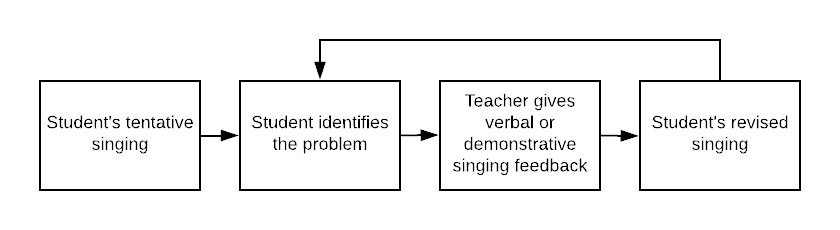
\includegraphics[width=\textwidth]{figs/blockDiags_rong/ch3_occurrance_flow.png}
\caption{The flowchart of a single correction occurrence.}
\label{fig:ch3_occurrance_flow}
\end{figure}

After five months research stay in NACTA (National Academy of Chinese Theatre Arts, leading institute in China dedicated to the training of professionals in performing and studying traditional Chinese opera), we had a firsthand experience of the month/heart teaching method of jingju singing. In class, the teacher teaches several melodic lines selected from an aria. In the first part of the class, the teacher gives a short introduction to the teaching content such as the story and the character setting of the aria, the special pronunciations. Then she/he gives a demonstrative singing of these lines. In the second part of the class, the students imitate the demonstrative singing line by line, and the teacher corrects the imitations. The process of the second part can be generalized as (i) the teacher asks the students to give a tentative singing individually at melodic line-level, or syllable-level. (ii) Then the teacher identifies the singing problems, (iii) gives verbal or demonstrative singing feedback. (iv) Finally, the students do a revised singing with the feedbacks in mind. The step from (ii) to (iv) could be iterated until the student's singing satisfies the teacher's criteria. We name one single such process as a correction occurrence (see \figref{fig:ch3_occurrance_flow}).

The verbal feedback is a semantic comment given by the teacher. It is the description that is aimed to help the student to improve her/his singing performance, and it is the most valuable information which can clarify the singing problems.

In paper \cite{geringer_musicians_1998}, the musicians have rated the performance of western arias in 5 musical dimensions: phrasing/expression, intonation, rhythm, loudness, tone quality. In our study, we borrow the concept of musical dimensions for music performance assessment and adapt them according to jingju singing background. 

Almost all jingju aria contains lyrics, and as we will prove in later chapters -- to be able to pronounce the singing lyrics accurately is a key skill in jingju singing, we thus add the pronunciation as an independent dimension to the dimension set mentioned above. Besides, we discard phrasing/expression because it is a ``meta-dimension" constructed above other basic dimensions -- ``A musician accomplishes this by interpreting the music, from memory or sheet music, by altering tone, tempo, dynamics, articulation, inflection, and other characteristics"\footnote{\url{https://en.wikiquote.org/wiki/Musical_phrasing} Retrieved 25 July 2018}. Overall, 5 dimensions will be taken into account in this paper -- intonation, rhythm, loudness, tone quality and pronunciation. Accordingly, we give their definitions:

\begin{itemize}
	\item Intonation: accuracy of pitch in singing.
	\item Rhythm: singing a rhythmic pattern on time, which means that the notes or syllable are not ahead of the time or behind the time.
	\item Loudness: the dynamic loudness variation between notes/syllables or phrases.
	\item Tone quality: the color or timbre of the singing voice.
	\item Pronunciation: the act or result of producing the sounds of speech, including articulation and stress.
\end{itemize}

In the next section, we explain our methods -- classifying teachers' correction occurrence and surveying the students. These methods aim to answer the question: how teachers and students value the importance of each jingju singing dimensions -- intonation, rhythm, loudness, tone quality and pronunciation. By classifying the correction occurrences, we will find out the dimensions on which teachers lay stress or students tend to have problems. On the other hand, we conduct a simple survey to investigate the importance of each dimension from the students' perspective.

\begin{figure}[ht!]
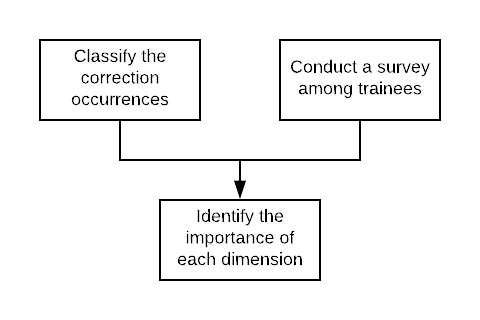
\includegraphics[width=\textwidth]{figs/blockDiags_rong/ch3_occurrance_analysis_flow.png}
\caption{The flowchart of the dimension importance identification process.}
\label{fig:ch3_occurrance_analysis_flow}
\end{figure}

\subsubsection{Correction occurrence analysis}\label{sec:ch3:correction_analysis}

During the research stay in NACTA, we audited and recorded the audio from three singing classes. Three class was taught respectively by three professional teachers, which contain solo and chorus practices. We recorded the class teaching and practicing audio content by using a SONY PCM-D50 stereo portable audio recorder. Only the solo practices are kept for the analysis because they can reveal the singing problems of an individual student, whereas the individual voices are blurred in the chorus practice recordings. The audio excerpts of each correction occurrence are then edited and visualized by signal processing tools—pitch contour, loudness contour and spectrogram, which is helpful in identifying the singing problem, especially when the teacher's verbal feedback is too abstract to extract any effective information. 

\begin{table}[ht!]
\centering
\begin{tabular}{ccccc}
\toprule
Aria name              & Role-type     & \makecell{\#Student} & \makecell{\makecell{\#Melodic\\line}} & \makecell{\makecell{\#Correction\\occurrence}} \\
\midrule
\makecell{武家坡\\WuJiaPo}          & laosheng & 3              & 11                  & 20                           \\
\makecell{太真外传\\TaiZhen\\WaiZhuan} & qingyi   & 3              & 3                   & 21                           \\
\makecell{捉放曹\\ZhuoFang\\Cao}      & hualian  & 2              & 28                  & 21                       \\
\bottomrule
\end{tabular}
\caption{The statistics of the correction occurrence analysis materials.}
\label{tab:correction_occurrence_stat}   
\end{table}

\tabref{tab:correction_occurrence_stat} depicts the information of aria name, role-type, student number in the class, melodic line number practiced in the class and correction occurrence number collected from the recordings. An example of reading this table is ``Three students were involved in the laosheng class WuJiaPo. 11 melodic lines were taught, and 20 correction occurrences were collected from the recordings".

The ratios between the melodic line number and the correction occurrence number are widely different for the three classes (\tabref{tab:correction_occurrence_stat}). For example, during the TaiZhenWaiZhuan class, three students practiced three lines and were corrected 21 times, which results in a ratio of 1/7. However, during the ZhuoFangCao class, two students practiced 28 lines and also were corrected 21 times, which has a ratio of 4/3. The correction frequency depends on several factors, such as the students' singing levels, the teacher's teaching method. The low singing level students tend to receive more corrections than those who have high singing levels.

For each occurrence, we analyze the target recordings and the teacher's verbal feedback. Additionally, to achieve the visual analysis, their pitch, loudness contours and spectrogram are also presented.

We firstly classify the correction occurrences into five dimensions—intonation, rhythm, loudness, tone quality and pronunciation. A correction occurrence can be classified into more than one dimension. For example, the correction with the verbal feedback “don't be sloppy, sing it with solidity, make the tone quality sounds round.” can be classified into intonation (irregular vibrato), loudness (unstable loudness contour) and tone quality (higher harmonics too clear), by analysing comparatively between the teacher's demonstrative singing and student's tentative singing. Furthermore, a finer inspection of each correction occurrence is conducted, where we identify the detailed elements.

Five correction occurrences are taken as examples to showcase our analysis. For each one, we list its aria name, melodic line, target syllable, the teacher's verbal feedback, the dimensions classified. Finally, we give a short explanation accompanied by the visualization to justify our classification process.

\begin{figure}[ht!]
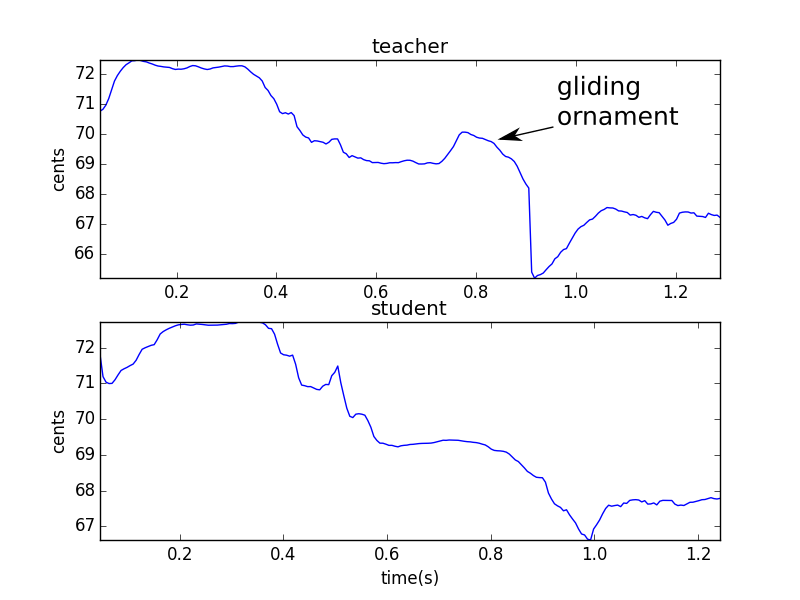
\includegraphics[width=\textwidth]{figs/spectro_vis/ch3_occ1.png}
\caption{The pitch contours of the syllable ``yuan" for occurrence 1.}
\label{fig:occurrence_1}
\end{figure}

\noindent\textbf{Occurrence 1:}

\begin{itemize}[leftmargin=*, noitemsep]
\item Aria: TaiZhenWaiZhuan (太真外传)
\item Line: yi yuan na chai yu he qing yuan yong ding (一愿那钗与盒情缘永定)
\item Target syllable: yuan (缘)
\item Teacher's verbal feedback: it didn't jump up. (没跳起来) 
\item Dimension: intonation
\item Explanation: The syllable's second tone in the teacher's demonstrative singing has a pitch gliding (ornament). However, the gliding in the student's version is not apparent (\figref{fig:occurrence_1}).
\end{itemize}

\begin{figure}[ht!]
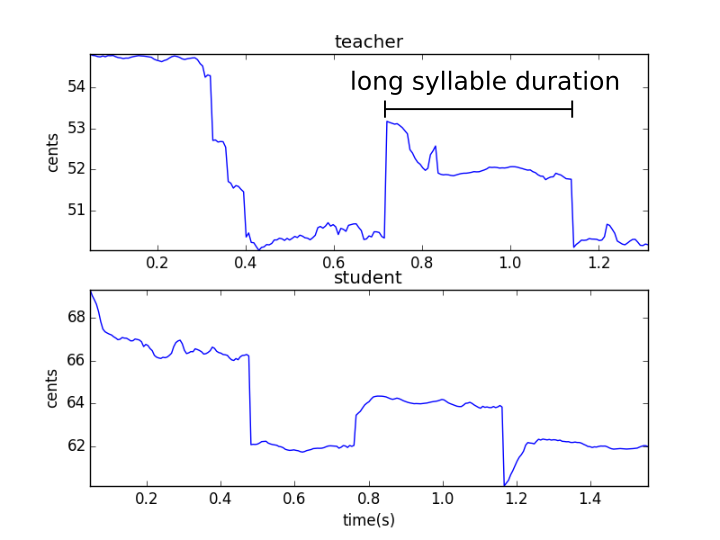
\includegraphics[width=\textwidth]{figs/spectro_vis/ch3_occ2.png}
\caption{The pitch contours of the syllables ``dang nian jie bai" for occurrence 2.}
\label{fig:occurrence_2}
\end{figure}

\noindent\textbf{Occurrence 2:}

\begin{itemize}[leftmargin=*, noitemsep]
\item Aria: ZhuoFangCao (捉放曹)
\item Line: dang nian jie bai yi lu xiang (当年结拜一炉香)
\item Target syllables: dang nian jie bai (当点结拜)
\item Teacher's verbal feedback: swing apart these four syllables (1,2,3,4 四个字甩开)
\item Dimension: rhythm
\item Explanation: In teacher's demonstrative singing, the temporal duration of the third syllable ``jie" has been prolonged, in contrast with the other three syllables, which can be observed by the pitch contour (\figref{fig:occurrence_2}).
\end{itemize}

\begin{figure}[ht!]
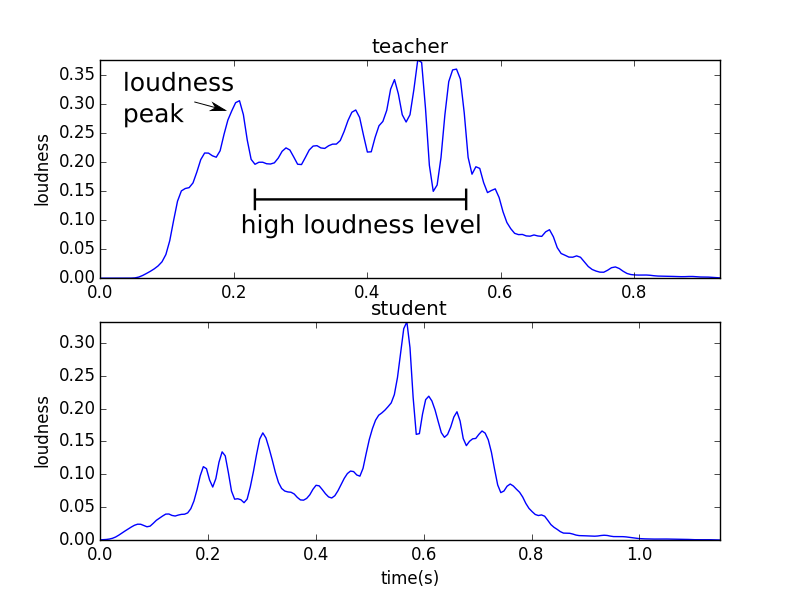
\includegraphics[width=\textwidth]{figs/spectro_vis/ch3_occ3_1.png}
\caption{The loudness contours of the syllable ``yang" for occurrence 3.}
\label{fig:occurrence_3_1}
\end{figure}

\begin{figure}[ht!]
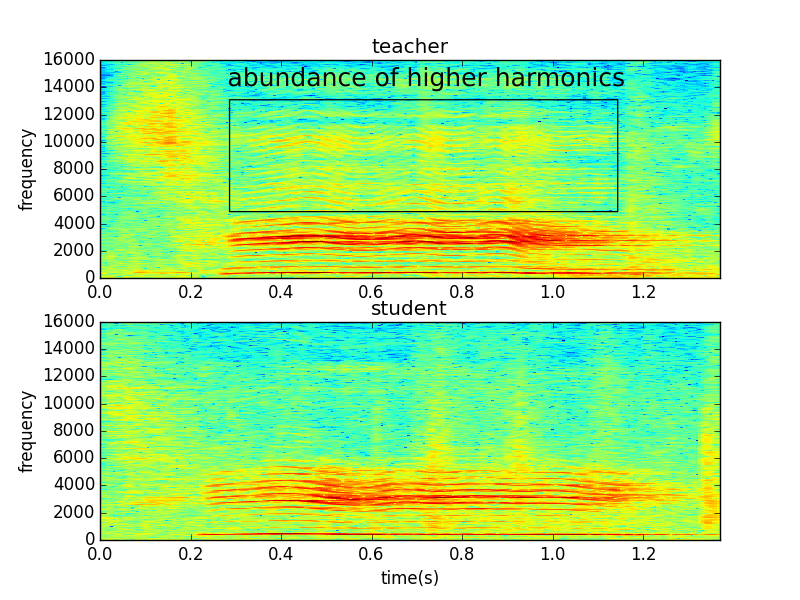
\includegraphics[width=\textwidth]{figs/spectro_vis/ch3_occ3_2.png}
\caption{The spectrograms of the syllable ``yang" for occurrence 3.}
\label{fig:occurrence_3_2}
\end{figure}

\noindent\textbf{Occurrence 3:}

\begin{itemize}[leftmargin=*, noitemsep]
\item Aria: TaiZhenWaiZhuan (太真外传)
\item Line: yang yu huan zai dian qian shen shen bai ding (杨玉环在殿前深深拜定)
\item Target syllable: yang (杨)
\item Teacher's verbal feedback: emphasizing the nasal voice (an 鼻音要突出)
\item Dimensions: loudness and tone quality
\item Explanation: In teacher's demonstrative singing, a prominent loudness peak can be found in the head of the syllable, which maintains a high loudness level in the belly (\figref{fig:occurrence_3_1}). We also can observe that the higher harmonics are abundant from the spectrogram (\figref{fig:occurrence_3_2}).
\end{itemize}

\begin{figure}[ht!]
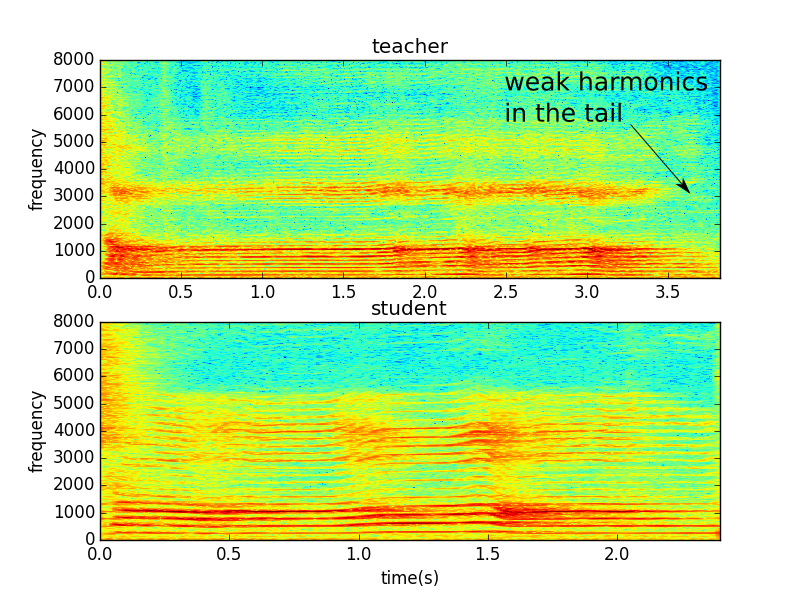
\includegraphics[width=\textwidth]{figs/spectro_vis/ch3_occ4.png}
\caption{The spectrograms of the syllable ``shang" for occurrence 4.}
\label{fig:occurrence_4}
\end{figure}

\noindent\textbf{Occurrence 4:}

\begin{itemize}[leftmargin=*, noitemsep]
\item Aria: ZhuoFangCao (捉放曹)
\item Line: xian xie zuo le na wa shang shuang (险些做了那瓦上霜)
\item Target syllable: shang (上)
\item Teacher's verbal feedback: terminate the sound at /ng/ (sound收音收到 ng)
\item Dimension: pronunciation
\item Explanation: The teacher's demonstrative singing is one octave lower than the student's singing. The teacher's feedback emphasizes the pronunciation quality of the syllable tail sound -- /ng/. His demonstrative singing contains fewer harmonics in the tail than the student's singing (\figref{fig:occurrence_4}).
\end{itemize}

\begin{figure}[ht!]
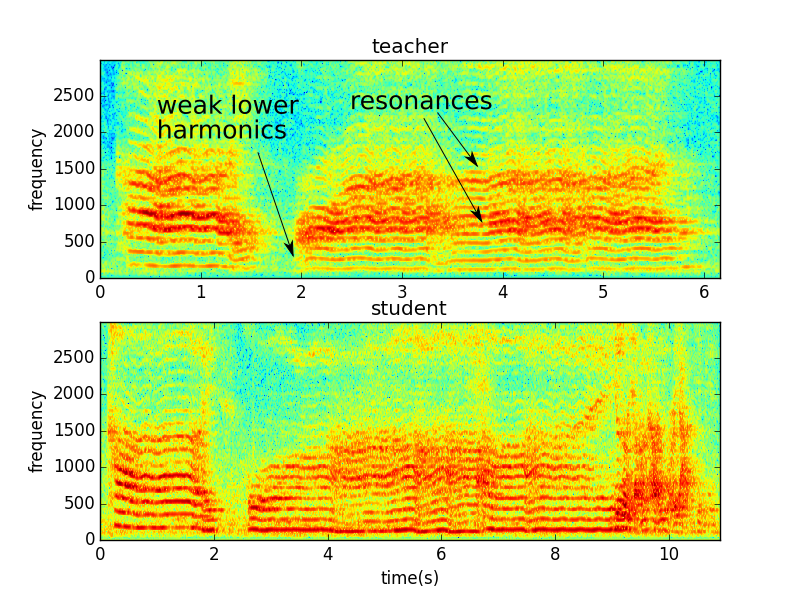
\includegraphics[width=\textwidth]{figs/spectro_vis/ch3_occ5.png}
\caption{The spectrograms of the syllables ``kai huai" for occurrence 5.}
\label{fig:occurrence_5}
\end{figure}

\noindent\textbf{Occurrence 5:}

\begin{itemize}[leftmargin=*, noitemsep]
\item Aria: WuJiaPo (武家坡)
\item Line: jian liao na zhong da sao xi wen kai huai (见了那众大嫂细问开怀)
\item Target syllable: kai huai (开怀)
\item Teacher's verbal feedback: adjust the breath, make the sound solid even if you sing in the low register (要用气,低调们也要放实在了)
\item Dimension: tone quality
\item Explanation: This feedback has twofold of meaning. First is to take enough breath, and have enough air in the chest to sing. Second is to adjust the body's resonance position to make the sound more solid. This can be observed as in the spectrogram of the teacher's demonstrative singing, which contains less energy for the lower harmonics and the prominent resonances (energy) in around 750 Hz and 1250 Hz (\figref{fig:occurrence_5}).
\end{itemize}

\subsubsection{A survey among students}
We conduct a simple survey of another nine students to investigate the importance of each dimension from their perspectives. The survey contains two questions: 

Please rate the use frequency of the following media when you learn to sing arias -- score, audio recording or teacher's classroom teaching. 
Please rate the importance of the following jingju singing dimensions and elements when you learn to sing arias—intonation, rhythm, loudness, pronunciation, ornament, breath and strength (劲头). 

Nine students have participated in this survey; they are different from the ones presented in \secref{sec:ch3:correction_analysis}. Among them, five are professional undergraduate students or students already graduated from NACTA, four are amateurs from the jingju associations in two non-art universities in Beijing. We use a five-level Likert scale for each rating term. For example, the ``use frequency of the score" in the first question and the ``importance of intonation" in the second question can be rated from 1 to 5, where 1 means ``never used" or ``not important at all" and 5 means ``most frequently used" or the ``most important". Then, we take the average value of each term for five professional students and four amateurs respectively. 

It is worth to mention that three more elements -- ornament, breath and strength have been added to the survey. The consideration for this change is that the survey terms need to be adapted to the student's artistic background, and the jingju singing jargons should be easily accessible by them.

\subsection{Results and discussion}

In this section, we report the results of the analysis of teachers' correction occurrences and the students' survey. The correction occurrences are classified into five dimensions by using the method introduced in the \secref{sec:probdef:correction_occurance}. Then, we discuss the student' survey result and compare it with the teachers' correction occurrence classification result.

\subsubsection{Correction occurrence analysis}\label{sec:ch3:correction_occurrence_results}

\begin{table}[ht!]
\centering
\begin{tabular}{cccccc}
\toprule
              & Inton.     & Rhythm & Loud. & Pronun. & \makecell{Tone\\quality} \\
\midrule
\makecell{武家坡\\WuJiaPo}          		& 8 	& 0 & 1 	& 6		& 6 \\
\makecell{太真外传\\TaiZhen\\WaiZhuan} 	& 6   	& 1 & 9 	& 4     & 11 \\
\makecell{捉放曹\\ZhuoFangCao}      		& 5  	& 2 & 7 	& 9     & 3 \\
Sum 									& 19 	& 3	& 17 	& 19	& 20 \\
\bottomrule
\end{tabular}
\caption{The statistics of the correction occurrence dimension classification. Inton.: intonation; Loud.: loudness, Pronun.: pronunciation.}
\label{tab:correction_occurrence_dimension_classification}   
\end{table}

We observe from the \tabref{tab:correction_occurrence_dimension_classification} that among the five dimensions, tone quality, pronunciation and intonation dimensions have the largest and almost equal occurrence number, loudness takes the second place, and rhythm problem was least mentioned. In other words, tone quality, pronunciation and intonation are the dimensions which receive particular attention from teachers and cause problems easily to students.

The correction occurrence analysis results are organized in an Excel spreadsheet, which consists of the teacher's verbal feedback, signal analysis method, and classified dimension.

\subsubsection{The survey among students}

We gather the survey results by ordering the mean values for each question. For the first question, the usage frequency ordered from high to low of three learning media are: 

\begin{enumerate}[noitemsep]
\item Professional group: classroom teaching, audio recording, score;
\item Amateur group: audio recording, teacher's classroom teaching, score. 
\end{enumerate}

The music score has been rated as the lowest use frequency by both professional and amateur groups, which means that the jingju students we investigated do not use the visual clue -- music score reading, to learn arias. The teacher's classroom teaching has been rated as the highest use frequency for the professional and the second for the amateurs, which is reasonable because this learning medium is much easier available for the professional. Lastly, the high rating of both teacher's classroom teaching and audio recording shows that the jingju students use mostly the listening and imitation methods to learn arias.

For the second question, the importance order from the most important to most trivial are: 

\begin{enumerate}[noitemsep]
\item Professional group: rhythm, strength, pronunciation, breath, intonation, loudness, ornament; 
\item Amateur group: rhythm, pronunciation, strength, ornament, breath, intonation, loudness. 
\end{enumerate}

Apart from the terms strength and breath, the others have been analyzed in the correction occurrence perspective. Strength is a stylistic and abstract word to depict the energy used in jingju singing and instrument playing. A jingju singing with strength is conveyed by combining multiple elements, such as loudness (mostly), rhythm, intonation and tone quality. Breath or specific methods of breathing (气口) described in Wichmann's book \cite{Wichmann1991a} is ``these methods allow the exiting breath to control the pitch, timbre or tone color, and energy of the sound produced." In consequence, Strength and breath both are nonspecific terms combining or affecting multiple basic jingju singing elements.

Pronunciation is rated as an essential element by both the professional and amateurs, which is coherent with the result of the correction occurrence analysis. The high importance of rhythm and low importance of intonation and loudness contradict to the result of the correction occurrence analysis. For rhythm aspect, one possible explanation is that the higher importance the students value a singing dimension, less prone they are going to sing poorly on it. For example, the students consider that rhythm is the most important singing aspect, they pay much attention to it during the practice. Thus they are less prone to have the rhythmic problems. For intonation and loudness, we cannot easily conclude that they are not important in the learning process. The reasons are twofold: on the one hand, the students might think that the intonation accuracy is a basic requirement in jingju singing and its importance is self-evident; on the other hand, because intonation and loudness are jargons used in acoustic, sound and music technology research fields, which might be foreign to these students, so they might avoid them and choose the familiar terms such as strength.

The only jingju singing dimension emphasized in both correction occurrence analysis, and the survey analysis is pronunciation, which shows that its crucial role in jingju singing training. As a consequence, to take advantage of limited time and effort, we will focus on tackling the research problems related to the assessment of singing pronunciation. In the following sections of this chapter, we present challenges, opportunities and research problems which are only related to the pronunciation dimension.

\section{Challenges and opportunities}

Significant challenges are existed to the automatic assessment of singing voice pronunciation in jingju music. We present and discuss challenges and opportunities from the perspectives of jingju singing characteristics and state of the art. These challenges will help us to formulate the research problems to be more comprehensive and akin to jingju music tradition. The opportunities, in turn, help us to pursue new MIR research directions. 

\subsection{Characteristics of jingju singing}\label{sec:ch3:char_singing}

We illustrate some signal characteristics of jingju singing voice that will be helpful to identify challenges for automatic assessment. 

\begin{landscape}
\mbox{}\vfill
\begin{figure}[ht!]
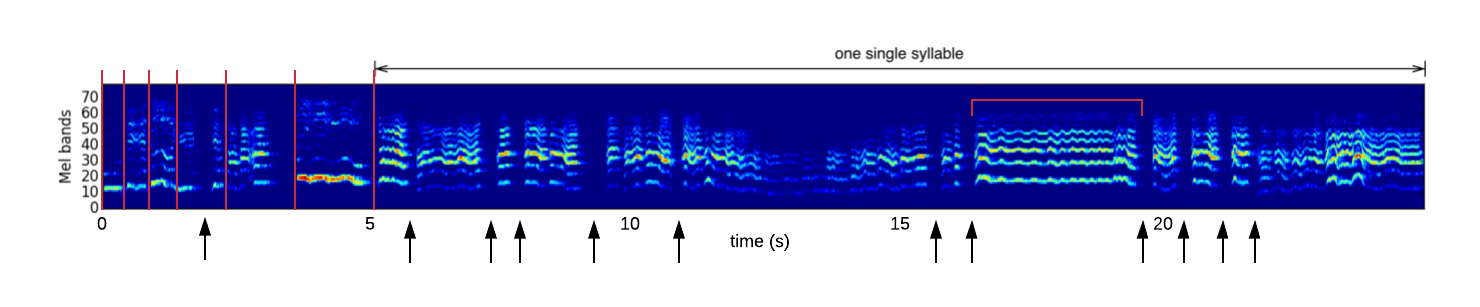
\includegraphics[width=1.8\textwidth]{figs/spectro_vis/ch3_jingju_char.png}
\caption{An example of a dan role-type singing phrase. Red vertical lines indicate the syllable onset time positions. Black arrows at the bottom specify the time positions of pause within the syllable. Red horizontal bracket shows a prominent singing vibrato.}
\label{fig:jingju_char}
\end{figure}
\vfill
\end{landscape}

\figref{fig:jingju_char} shows an example of a \textit{dan} role-type singing phrase in which the last syllable lasts approximately 20 seconds. This singing method -- 拖腔 (pinyin: tuoqiang, literally translated as the prolonged melody), used more commonly in \textit{dan} than in \textit{laosheng} singing, extends the duration of last syllable of the melodic line or a dou (\secref{sec:ch2:lyrics_structure}). It is a way of improving artistic expression, and the prolonged syllable can be used to carry various singing skills which include breath, intonational and dynamic control techniques, among others. 

In jingju singing, the breath must be under purposeful control at all times \cite{Wichmann1991a}. 偷气 (pinyin: touqi, stealing breath) is one of the primary methods to taking the breath in jingju singing. Performer inhales rapidly without exhaling beforehand. Touqi is performed when a sound is too long to be delivered in one breath and should be undetectable to the audience \cite{Wichmann1991a}. However, this is not the only technique which can lead to pauses within a syllable. Another singing technique (\textit{zu yin}, literally translated as block sound), provokes also pauses without occurring exhalation or inhalation. This kind of pause can be very short in duration and can be easily found in jingju singing syllables. 

Vibrato (颤音 chanyin and 波浪音 bolangyin) is extremely important in jingju singing such that a single pitch is rarely prolonged without a vibrato. Compared to the Western opera, jingju singing vibrato is slower and wider regarding vibrato rate and extent \cite{Yang2015a}.  

\begin{figure}[ht!]
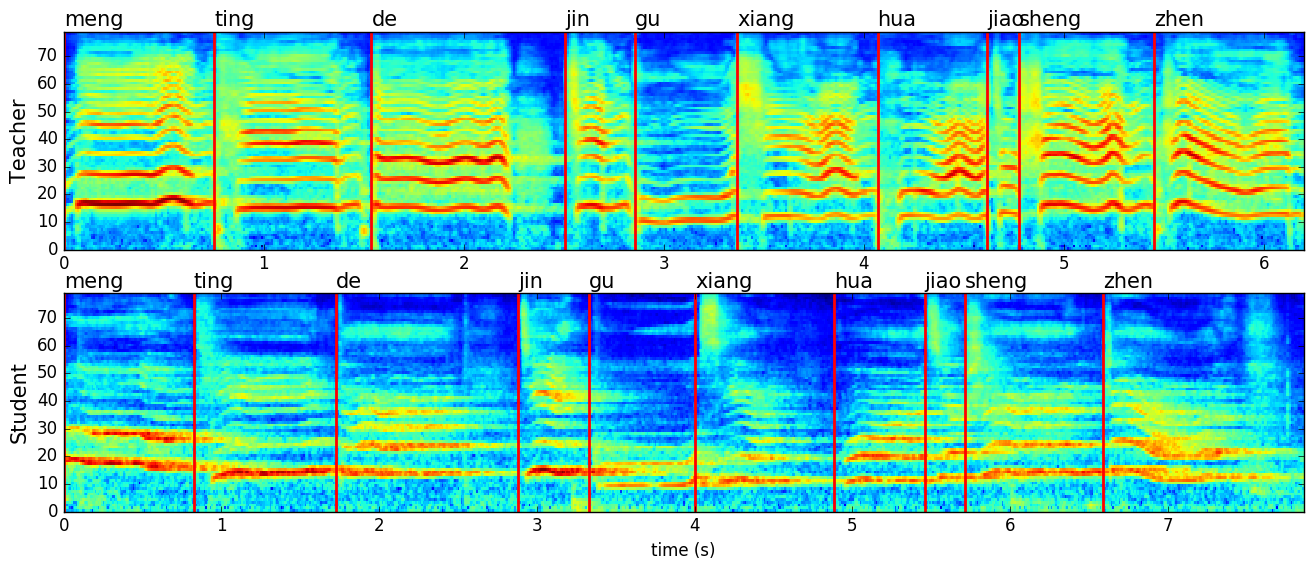
\includegraphics[width=\textwidth]{figs/spectro_vis/ch3_overall_qua.png}
\caption{The Mel spectrograms of teacher and student singing the same phrase ``meng ting de jin gu xiang hua jiao sheng zhen (in pinyin format)". Red vertical lines are the onset time positions of each syllable.}
\label{fig:overall_qua}
\end{figure}


The overall quality of the singing syllable or phoneme can be easily illustrated by using spectrogram. \figref{fig:overall_qua} shows the Mel spectrograms of a dan role-type singing phrase taken from the aria 猛听得金鼓响画角声震--《霸王别姬》 (meng ting de jin gu xiang hua jiao sheng zhen -- Farewell My Concubine). The upper part of the figure is the spectrogram of the teacher's recording, while the lower part is that of a primary school student's recording. Although the student does not commit any mispronunciation, there still exists a significant gap between the overall quality of her singing and that of the teacher singing. The gap is reflected in many aspects if we compare the two spectrograms. For example, the higher harmonics of the student singing is much weaker than those of the teacher; The consonants energies of the student singing are weaker than those of the teacher if we compare the consonants of syllables ``xiang" and ``sheng"; The intonation of the student singing is flat and lacks variation. 

\subsection{Challenges}\label{sec:ch3:challenges}

The basic music event of jingju singing is syllable. In jingju singing training, the accurate rendition of the syllabic pronunciation is placed in a more important position than that of the melody. In jingju circle, there is a saying 依字行腔 (pinyin: yi zi xing qiang, literally translated as singing according to the syllables), meaning that the singing melody should be consistent with the syllable tone and pronunciation, which also shows the importance of an accurate syllabic pronunciation. In \secref{sec:ch2:jingju_syllable}, we presented the structures and the lower-level components of jingju singing syllable. A jingju singing syllable consists of four types of phoneme -- an initial consonant or semivowel (optional), a medial vowel (optional), a central vowel and a tail (optional). As a consequence, at a more elaborate level, to pronounce a jingju syllable accurately is to render these elementary phonemes accurately.

According to the jingju singing principles mentioned above, to assess a jingju singing pronunciation at syllable or phoneme level, an automatic assessment system of jingju singing needs to have the ability to segment the singing recording automatically into the syllabic or phonetic unit. As we have mentioned in \chapref{chap:bkgnd}, a jingju aria is arranged hierarchically in several granularities from the roughest to the finest -- banshi, couplet (shangxiaju), melodic line, syllable. Ideally, the segmentation of a jingju singing in a certain granularity needs to be performed on top of its parent one. For example, the segmentation of couplet needs to be done in its parent banshi segment; the segmentation of syllable needs to be done in its parent melodic line segment. Correspondingly, if the target recording for the assessment is an entire aria, which is required to be assessed in syllable or phoneme level, we need systems for different segmentation granularities -- automatic banshi, couplet, melodic line, syllable and phoneme segmentation. 

One way to approach the segmentation problem of different granularities is the alignment of aria lyrics to audio. Since lyrics can be annotated with boundaries of banshi, couplet and melodic line, once each syllable in the lyrics are time-aligned with the singing audio, the time boundaries of different granularities can be naturally deduced. However, this unified approach might not be optimal regarding the segmentation accuracy. Different banshi has the different singing characteristic. For example, prolonged singing syllables are more likely to be sung in unmetered banshi segments, such as \textit{daoban} and \textit{huilong}, and in slow temp banshi, such as manban. As it was mentioned in \secref{sec:ch3:char_singing}, many singing skills such as ornamentation, breath control, are usually used in interpreting a prolonged syllable. Breath control leads to silences within a syllable; ornamentation leads the variation of the spectral pattern. Long syllable, silences within a syllable and spectral pattern variation are the main sources of lyrics-to-audio alignment error. Thus, to avoid the alignment error propagating in different banshi segments, it is necessary to perform the banshi segmentation.

Different tempi and meters characterise different banshi (\secref{sec:banshi}). Thus banshi segmentation is analogous to meter tracking \cite{Srinivasamurthy2016}. Unmetered banshi is an important category of jingju banshi of which the singing and instrumental performing do not follow any rhythmic beat. Such unmetered banshi existing in jingju aria present challenge to the segmentation task.

Jingju music tradition does not have the absolute tempo. An expressive performance without a metronome, combined with a lack of annotated tempo can lead to a single composition being performed in different tempi. This lack of an absolute tempo complicates the choice of a relevant timescale for tracking banshi \cite{Srinivasamurthy2016}.

The jingju music characteristics allow a certain freedom of improvisation in changing the local tempo such as increasing or decreasing the tempo through the melodic line or a few syllables. However, MIR algorithm has difficulty tracking metrical structures that have expressive timing and varying tempo \cite{Holzapfel2012a}. Thus, the local tempo variation is a potential source of challenge for banshi tracking.

Regarding segmentations in finer granularities than banshi, as we have mentioned above, long syllable, silences within a syllable and spectral pattern variation pose challenge to the relevant segmentation/alignment tasks. 

mispronunciation challenges

Pronunciation and overall quality of a singing syllable or phoneme are both abstract and perceptual related concepts. Pronunciation is a subconcept of the timbre which is defined by what is not ``a set of auditory attributes of sound events in addition to pitch, loudness, duration, and spatial position". In a signal point of view, timbre is related to the spectral envelope shape and the time variation of spectral content \cite{Pons2017Timbre}. While overall quality is a more general concept than pronunciation since it is a mixture of different musical dimensions -- intonation, loudness, duration and timbre (apart from pronunciation). In consequence, to define a pronunciation similarity measure requires a perceptual related representation of the time-varying spectral content, and to define an overall quality similarity measure requires a representation of all relevant dimensions. To identify the proper representations for similarity measures is a potential challenge.

In summary, the absence of an absolute tempo and local tempo variation are challenging. Long syllable, silences within a syllable and spectral pattern variation pose challenges to existing segmentation approaches. The fuzziness of pronunciation and overall quality concepts present challenges in finding proper representations for their similarity measurement.

\subsection{Opportunities}

There are several unique features in jingju singing which bring new opportunities to explore new research directions in MIR. The challenges mentioned above also bring new opportunities to explore new approaches for automatic singing voice assessment. The complex metrical structure and syllable-based singing framework requires specific methodologies to perform segmentation and pronunciation description, and will be beneficial to the singing assessment of other music cultures based on similar frameworks.

In this dissertation, we mainly use audio for analysis. However, the corresponding score, lyrics and annotated metadata which also carry pronunciation and duration information can be used for a compound approach for building the singing assessment models.

Another important aspect of jingju singing is that its pronunciation is explicitly shown through the shapes for the throat and mouth (\secref{sec:ch2:sihu_wuyin}). In jingju singing training, students are required to use a standardized throat and mouth shape to pronounce jingju syllables. It is believed a non-standard throat and mouth shape cannot lead to the correct pronunciation. Thus, a multi-modal approach to jingju singing pronunciation assessment can be done from video recordings of student singing practice, a problem is interesting, but beyond the scope of this dissertation.

The language system of jingju singing is a variant of the standard Mandarin Chinese. Although various Chinese dialects are used in jingju singing and bring certain variations to Mandarin pronunciation, such as special pronunciations -- shangkouzi, the syllabic structure of Mandarin language remains unchanged (\secref{sec:ch2:jingju_syllable}). We can learn methodologies from the mature research area of speech technologies to resolve segmentation and mispronunciation detection problems. 

In summary, the unique metric structure, syllable-based singing framework and variants of Mandarin language bring new opportunities for exploring new methods in jingju singing. Additionally, a detailed description of jingju singing pronunciation involves combining various sources of information such as audio, score, lyrics, annotated information related to pronunciation and visual cues.

\section{Research problems in the assessment of singing voice pronunciation of jingju music}

We have identified so far several challenges and opportunities for automatic assessment of singing pronunciation in jingju music. With such context, we will describe relevant research problems, discuss possible methods, and review existing works for each problem. Some associated problems not directly tackled in this dissertation such as banshi segmentation, are also discussed for completeness. Many of the singing assessment problems for jingju singing have not been tackled before, whereas similar problems in speech or other music traditions have been aimed to resolve in speech technology or MIR fields. Most of the tasks for assessment of jingju singing pronunciation need to be reformulated with the jingju singing background such as onset detector is regarded as useful to develop specific syllable/phoneme segmentation algorithm with the help of other sources of information.

\begin{figure}[ht!]
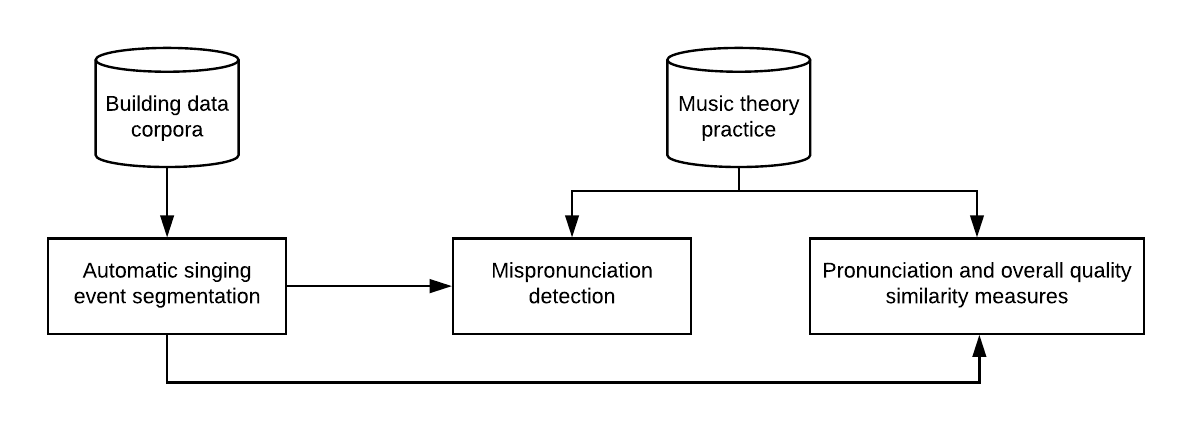
\includegraphics[width=\textwidth]{figs/blockDiags_rong/ch3_related_topics.png}
\caption{Related research topics of automatic assessment of singing voice pronunciation in jingju music.}
\label{fig:related_research_topics}
\end{figure}

In this dissertation, the assessment of singing pronunciation will be devised at syllable or phoneme level. There are several sub-problems which lead to the final goal -- to develop mispronunciation detection models and to define pronunciation similarity measure for jingju singing. In \figref{fig:related_research_topics}, we show the information flow between four topics of research problem that will be addressed in this dissertation -- building data corpora, automatic singing event segmentation, mispronunciation detection and pronunciation and overall quality similarity measures. There is a significant sequential order while addressing each problem, e.g. to achieve the assessment at syllable or phoneme level, mispronunciation detection and similarity measures benefit from the results of automatic singing event segmentation. The topics of mispronunciation detection and similarity measures use knowledge derived from music theory and practice, making them more culture-aware. Each of the topics will be discussed in detail.

\subsection{Building data corpora}

A crucial part of data-driven research using machine learning approaches requires good quality data. Data corpora of the music tradition under research are crucial for building and testing the automatic assessment models. The data should contain various sources such as audio, score, lyrics and manual annotation made for automatic assessment research.

The dataset created in the work \cite{repetto_creating_2014} is formed by a collection of commercial recordings, as well as their metadata. Another jingju music corpus gathered in the \cite{Tian2016} also consists of commercial recordings, and annotated for structural segmentation analysis. These recordings are all mixed with instrumental accompaniment, which means a cappella (clean) singing voice should be separated during the preprocessing step if we want to make use of these recordings for the research of automatic assessment. A collection of 92 jingju music scores gathered for the analysis of jingju musical system is presented in the work \cite{Repetto2017}, which is transcribed from published books and stored in machine-readable format. The a cappella singing separated commercial recording dataset and the modified score dataset will be integrated into the data corpora of this dissertation.

The a cappella jingju singing dataset created in the work \cite{black_automatic_2014} consists of 31 unique arias in total around 1-hour recordings. However, due to the small size of this dataset, and that its annotations were made for the task of mood recognition rather than automatic assessment, we have to re-annotate this dataset firstly, and then expand it to a proper scale. One of the main problems tackled in this dissertation is building suitable and scalable data corpora for the singing pronunciation assessment research, a problem that is discussed further in \secref{sec:ch3:dataset_research}. 

\subsection{Automatic singing event segmentation}

Automatic singing event segmentation includes a set of problems that aim to infer or time align the boundaries of several musical events in singing recordings related to pronunciation assessment. The common MIR tasks such as musical structure segmentation, lyrics-to-audio alignment and singing event onset detection can be classified as automatic singing event segmentation problems. As we have mentioned in \secref{sec:ch3:dataset_research}, in the context of the assessment of jingju singing pronunciation, the relevant singing events to consider are banshi, couplet, melodic line, syllable and phoneme. 

Automatic singing event segmentation is an important preliminary step to achieve automatic assessment, and there are several applications in which the segmentations are useful, such as rhythm-based annotation of audio, beat/melodic line/syllable aligned processing of music, audio summarization. Each of these problems will be described in detail.

\subsubsection{Banshi segmentation}

Banshi segmentation (or banshi tracking) is not the problem which will be tackled in this dissertation. However, we discuss it for completeness. Banshi segmentation refers to a set of problems that focus on segmenting different banshi sections in a jingju aria. By segmenting the banshi sections, a complete description of jingju metrical structure can be achieved. For such a problem, the subcomponents of a banshi -- tempo, accented beat (ban or downbeat), unaccented beat (yan or beat) can be obtained.

Banshi segmentation can be done either in an uninformed or informed fashion. The former fashion means that inferring the time-varying tempo, beats and downbeats without any prior banshi knowledge of the aria. Informed banshi segmentation is the case to track tempo, beats and downbeats given the information of the banshi sequence of the aria. We can classify the subtasks as tempo tracking, beat tracking and downbeat tracking. Tempo tracking aims to estimate the time-varying tempo over the recording of a jingju aria. The tracked tempo will be useful for the beat tracking tasks. As we have mentioned in \secref{sec:ch3:dataset_research}, the tempo tracking method applied for jingju aria needs to be robust for the local or long-term tempo change. For metered banshi, the rhythmic beats are performed by several percussion instruments -- danpigu, ban, naobo, daluo and xiaoluo. Thus, the beat time instance is defined by the onset of each percussion instrument stroke. Although a specific beat tracking algorithm has not been developed for estimating metered jingju banshi, a suitable jingju percussion onset detection method \cite{Tian2014} and several beat tracking methods \cite{Bock2011, Krebs, Bock} for eurogeneric music can be adapted for this purpose. In jingju performance, each downbeat is usually marked by the ban (wooden clapper) sound and indicates the first beat a measure \cite{Wichmann1991a}. Thus downbeat tracking can be formulated as the problem of estimating the onset time positions of the ban sound in the beat sequence. Lastly, metered banshi tracking in jingju aria is a task analogous to tala tracking in Indian art music, of which the relevant methods have been studied extensively in Srinivasamurthy's work \cite{Srinivasamurthy2016}.

Due to the lack of tempo and beat, segmenting metered banshi requires a different framework mentioned above. Banshi segmentation is an important step towards any finer segmentation task of jingju aria. However, since we adopt the melodic line directly as the input of the assessment pipeline, banshi segmentation will not be a problem considered in this dissertation.

\subsubsection{Couplet, melodic line, syllable and phoneme segmentation}

Couplet or melodic line segmentation refers to estimate the time boundaries of singing couplet or melodic line in a banshi section. The syllable or phoneme segmentation aims to transcribe the audio recording of a melodic line into a time-aligned syllable or phoneme sequence. In jingju singing training scenario, the score, lyrics and relevant annotations such as starting and ending syllables of the couplet or melodic line are usually given beforehand. Thus, these problems can be formulated into a uniformed framework -- lyrics-to-audio alignment. Time-aligning lyrics to audio is a fine-grained segmentation task, which can be applied to the syllable or phoneme level singing assessment and analysis.

Jingju is sung in Chinese Mandarin language with regional dialect pronunciations of which each written character is pronounced as a syllable (\secref{sec:ch2:jingju_syllable}), and several written characters make up a word. Although not many languages in the world adopt the similar writing system, the pronunciation of all languages is built upon basic units -- phoneme and syllable \cite{Moran2014}. Thus the lyrics-to-audio alignment method can be devised as either language-dependent or language-independent. Both methods can be formulated as supervised learning tasks. The former uses label data to build syllable or phoneme models; while the latter uses labelled data to build syllable or phoneme boundary models.

As discussed in \secref{sec:ch3:challenges}, several jingju singing characteristics such as long syllable, silences within a syllable and spectral pattern variation pose challenge to the lyrics-to-audio alignment task. Apart from that, another challenge is that the mapping from the written characters to syllables is not unique, due to the existence of special pronunciations and multi-pronunciation characters in jingju singing.

The work on lyrics-to-audio alignment for jingju singing has been very limited so far. Dzhambazov et al. \cite{dzhambazov_modeling_2015} proposed a modified text-to-speech alignment method for jingju singing. The system is built upon a duration-explicit hidden Markov model, where the phoneme duration is empirically set according to lyrics and metric structures of jingju music.

It is to be noted that prior musical information such as score is usually available for the assessment of jingju singing, and can be exploited to tackle the related challenges. Lastly, since we adopt the melodic line directly as the input of the assessment pipeline, couplet or melodic line segmentation will not be a problem considered in this dissertation. Syllable and phoneme segmentation is one of the problems addressed in this dissertation and is formulated more concretely in \secref{sec:ch3:segmentation_formulation}.

\subsection{Mispronunciation detection}

mispronunciation detection for mandarin speech

\subsection{Pronunciation and overall quality similarity measures}

Pronunciation and overall quality similarity measures refer to build an objective model to calculate the similarity of corresponding jingju singing segments between teacher and student respecting pronunciation and overall quality aspects. The similarities can be measured in different singing granularities such as banshi section, couplet, melodic line, syllable and phoneme. In this dissertation, we tackle only the problem of building the models of phoneme-level pronunciation and overall quality similarity measures since phoneme is the finest grained pronunciation unit of jingju singing, and the composition basis of any higher singing granularities such as syllable, melodic line, couplet and banshi section. Likewise, phoneme is also the finest grained pronunciation unit of any other languages. The method developed in building similarity measures at phoneme-level in jingju singing can be easily adapted to singing similarity measurement at phoneme-level in any other languages. The application of such similarity measure is not limited to the assessment of singing voice. Other potential applications are the assessment of pronunciation at phoneme-level in the second language (L2) learning and broadcasting training. In such scenarios, the similarity between the phoneme segments of a language learner and a native speaker needs to be shown to give the learner a clue about how well her/his pronunciation or overall quality is. 

The challenge of this topic, as mentioned in \secref{sec:ch3:challenges}, is to find proper representations for similarity measures -- representation learning. Pronunciation is represented in the signal point of view as the time-varying spectral change. Overall quality is a perceptual concept mixed with different musical dimensions such as intonation, loudness, duration and timbre. The representations need to capture the time-varying and abstractive natures of these two concepts. The representation learning can be formulated as a supervised discriminative or a semi-supervised distance metric learning tasks. Take overall quality aspect as an example, a supervised discriminative learning uses labeled data (e.g. good/bad quality) to build a discriminative model, while a semi-supervised distance metric learning uses data labeled in pairwise or triple-wise similarity to build a model, e.g. the overall quality of samples A and B are similar; that of sample B and C are not similar. As a consequence, the learned representation from either the discriminative model or distance metric learning model is used for the similarity measurement.

We cannot identify any previous work on the topic of pronunciation or overall quality similarity measure at phoneme-level. However, there exist a significant amount of works on the topic of speech phonetic similarity applied in L2 learning. Minematsu et al. \cite{Minematsu2004, Minematsu2007, Shiozawa2016} propose a structural representation of speech phoneme sounds. They train HMM for each phoneme class, then compute Bhattacharyya distance between each HMM pairs. The pairwise distance matrix represents the phoneme-level linguistic structure. They also claim that this representation is represent purely the linguistic traits of a language and free from any distortion such as microphone, room, speaker. Thomson \cite{Thomson2008} develops a method to measure the English vowel similarity for Mandarin speaker. He builds discriminative models for each English vowel using the recordings of English native speakers, then uses the models to calculate the posterior probability as the similarity measure for vowel segment of Mandarin speakers. Wieling et al. \cite{Wieling2011} focus on the multidimensional scaling (MDS) representation of vowel segments. They use formant frequencies as the feature to calculate the euclidean distance for each vowel pair, then perform MDS to project each vowel onto a two-dimensional similarity space. Mielke \cite{Mielke2012} explores DTW distance for phonetic similarity measure. He uses MFCC as the representation of the phoneme segment, and compute DTW distance between two MFCC vectors. Kyriakopoulos et al. \cite{Kyriakopoulos2017} develop a phoneme similarity measure based on Jensen-Shannon divergence. They calculate aggregate PLP feature and fit multivariate Gaussian model for each phoneme. The Jensen-Shannon distance is computed on the multivariate Gaussian models of each phoneme pair.

Pronunciation and overall quality similarity measures are one of the problems addressed in this dissertation. A more comprehensive problem formulation will be presented in \secref{sec:ch3:similarity_formulation}.

\section{Formulation of thesis problems}

With an overview of the research problems, challenges, review of the state of the art works, a subset of those problems that will be tackled in this dissertation are defined. In this section, we formulate these problems more comprehensively by discussing their assumptions, restrictions, and objectives in an engineering way.

\subsection{Dataset for research}\label{sec:ch3:dataset_research}

Building a dataset for MIR research is a scientific problem. Objective criteria are set up for designing, curating and also measuring the goodness of a corpus. One of the goals of CompMusic project is to build such data corpora and make it available for the research usage. Collection of good quality data and easily accessible audio and metadata is crucial for the research reproducibility.

For developing relevant approaches, we focus on collecting and curating a cappella (clean) jingju singing voice audio in jingju singing training scenario. The jingju a cappella audio dataset includes both professional (teacher) singing audio and amateur (student) imitative singing audio, which accompanied with hierarchical jingju musical events annotations. For all of the tasks addressed in this dissertation, we need singing syllable and phoneme boundary annotations. Specifically, for mispronunciation detection task, we annotate special pronunciation singing syllables. 

In general, for the research of automatic assessment of jingju singing voice, we aim to build a data collection which can represent the real world singing training scenarios. The recordings need to include the main role-types disciplined in singing, common teaching repertoire. The datasets built in the context of this dissertation are further presented in Chapter 4.

\subsection{Syllable and phoneme segmentation}\label{sec:ch3:segmentation_formulation}

One of the problems addressed in this thesis is syllable and phoneme segmentation of jingju singing recordings. To the best of our knowledge, for jingju music, a system which can achieve a certain segmentation accuracy to be suitable for the needs of automatic assessment at syllable or phoneme level does not exist yet. Additionally, to improve the segmentation accuracy, we also explore incorporating a priori musical information such as the syllable or phoneme duration extracted from music scores or annotations into the segmentation algorithm.

To address the problem, we formulate tasks that can integrate a priori syllable or phoneme duration information -- duration-informed syllable and phoneme segmentation. The a priori duration information is extracted either from the musical score or manual annotation, which thus represents the coarse syllable or phoneme duration in the target recording. We then use data-derived audio representation indicative of syllable or phoneme onset events in the recording. Finally, we build hidden Markov models that can incorporate the a priori duration information into the syllable or phoneme boundary selection step. The onset detection-based rather than the forced alignment-based approach is used since the former is a binary classification task which requires less training data, and onset time stamps annotation is available for model training.

In the scope of this work, the target singing recording is assumed to have been already segmented into pieces that are in a single melodic line. This assumption mainly stems from the fact that in the actual jingju singing training course, the materials are taught and practised line by line. We do not assume any restrictions on banshi type over the melodic line. We restrict our work to two role-types -- dan and laosheng in jingju music. The restriction is mainly because dan and laosheng are respectively two major role-types of female and male singing styles, and that singing is the main discipline of these two role-types. The proposed method is likely to extend to the singing of other role-types, provided we have the a priori duration information for them. 

The a priori syllable durations of the target melodic line are stored in an array $M^s=\mu^{1} \cdots \mu^{n} \cdots \mu^{N}$, where $\mu^{n}$ is the duration of the nth syllable. The a priori phoneme durations are stored in a nested array $M_p=M^{1}_p \cdots M^{n}_p \cdots M^{N}_p$, where $M^{n}_p$ is the sub-array with respect to the nth syllable and can be further expanded to $M^{n}_p=\mu_{1}^{n} \cdots \mu_{k}^{n} \cdots \mu_{K_{n}}^{n}$, where $K_{n}$ is the number of phonemes contained in the nth syllable. The phoneme durations of the nth syllable sum to its syllable duration: $\mu^{n}=\sum_{k=1}^{K_{n}} \mu_k^{n}$. In both syllable and phoneme duration sequences -- $M^s$, $M_p$, the duration of the silence is not treated separately and is merged with its previous syllable or phoneme. Let the recording of a melodic line can be reduced by short-term Fourier transform (STFT). The goal is to find the best onset state sequence $Q={q_1 q_2 \cdots q_{N-1}}$ for a given syllable duration sequence $M^s$ or phoneme duration sequence $M_p$ and impose the corresponding syllable or phoneme label, where $q_i$ denotes the onset of the $i+1$th or the offset of the $i$th inferred syllable/phoneme.

The approaches, experiments and results for syllable and phoneme segmentation are presented in Chapter.

\subsection{Mispronunciation detection for special pronunciation}

\subsection{Pronunciation and overall quality similarity measures at phoneme level}\label{sec:ch3:similarity_formulation}

The problem of pronunciation and overall quality similarity measures is the fourth problem that will be addressed in this thesis. The approach we explore is to learn phonetic pronunciation and overall quality representations using representation learning techniques and compute the similarity between two representations using distance measure. The goal is to test the effectiveness of representation learning techniques in learning pronunciation or overall quality discriminative representations. Differ from the previous similarity measure approaches which use handcrafted features as the representation, and perform DTW related methods to compute the similarity between two variable-length features, we present an approach in this dissertation based on acoustic phoneme embeddings which map the variable-length phoneme segments into fixed-length vectors, which facilitate the similarity calculation.

We assume that the singing recordings have been segmented into phoneme units, which is done manually in this dissertation. Although the segmentation can be done automatically by using the approach presented in \secref{sec:ch3:segmentation_formulation}, this assumption can make sure the segmentation accuracy, and thus avoid the error propagated by the automatic segmentation step. We restrict in our work the overall quality to be a binary rubric such that phoneme segments sung by the teacher have a professional overall quality, and those sung by the student have an amateur overall quality. Thus, the overall quality similarity is measured between teacher and student phoneme segment pair which belong to the same phoneme class. For example, the approach can only measure the similarity between phoneme segments A and B, where A is sung by teacher and B is sung by student; A, B belong to the same phoneme class. From the point of view actual jingju singing training, only the case mentioned above is valid since the similarity between two phoneme segments sung consistently by teacher or student would not be measured, and measuring the similarity between two segments belonging to different phoneme classes is a problem which can be avoided by mispronunciation detection. Since we can be sure that the student recordings in our dataset can by no means reach the professional level, such a restriction is justified.

Let the set of variable-length phoneme segments be denoted as $\mathcal{A} = {A_1, A_2, A_3, ..., A_N}$, where each $A_j$ is a subset of phoneme segments belonging to class j. The learned phonetic pronunciation representation for each phoneme segment in $A_j$ should be capable of minimizing the intra-class similarity and maximizing the inter-class similarity. Let the set of variable-length phoneme segments sung by teacher be denoted as $\mathcal{B}={B_1, B_2, B_3, ..., B_{N}}$, and another set of variable-length phoneme segments sung by student be denoted as $\mathcal{C}={C_1, C_2, C_3, ..., C_{N}}$, where each $B_j$ and $C_j$ are the subsets of phoneme segments belonging to class j. The learned phonetic overall quality representation should be capable of minimizing the intra-class similarity between two segments from one single set such as B or C, and maximizing the inter-class similarity between those from different sets such as $B_j$ and $C_j$. 

The whole approach can be formulated as a fixed-length representation learning problem with pre-segmented phoneme samples -- using the fixed-length representation for the similarity computation. The approaches, experiments and results for syllable and phoneme segmentation are presented in Chapter.